% reality/realized_pose3-DE.tex
\chapter{Realisiertes pose3 und Ziel--Realisiert-Vergleich}
\label{chap:realized-pose3}

Dieses Kapitel verwendet die kanonischen pose3-Definitionen aus Grundlagen
und Zustand (\cref{def:pose3} und \cref{def:runtime-pose3}) und definiert die in
Realitätsabläufen verwendeten realisierten und gemessenen Gegenstücke.

\begin{principle}[Prinzip des realisierten Zustands]
\label{princ:realized-state-principle}
In AIM hängt die operative ingenieurtechnische Interpretation vom realisierten
Laufzeitzustand und nicht allein vom Zielzustand ab.
\end{principle}

\section{Ziel-, realisiertes und gemessenes pose3}

\begin{definition}[Ziel-pose3]
\label{def:target-pose3}
Der Zielzustand der Eisenbahn wird bezeichnet durch
\[
\mathrm{pose3}_{\mathrm{target}}(s).
\]
\end{definition}

\begin{definition}[Realisiertes pose3]
\label{def:realized-pose3}
Der realisierte Eisenbahnzustand wird bezeichnet durch
\[
\mathrm{pose3}_{\mathrm{real}}(s).
\]
\end{definition}

\begin{definition}[Gemessener pose3-Zustand]
\label{def:measured-pose3}
Ein gemessener pose3-Zustand ist eine aus Beobachtung abgeleitete Approximation
\[
\mathrm{pose3}_{\mathrm{meas}}(s_i)
\approx
\mathrm{pose3}_{\mathrm{real}}(s_i).
\]
\end{definition}

\begin{principle}[Prinzip der Messtrennung]
\label{princ:measurement-separation}
Zielzustand, realisierter Zustand und gemessener Zustand sind verschiedene
Ebenen.
\end{principle}

Die erste Abbildung beantwortet die Ebenenfrage unmittelbar: Wie sind Ziel-
und realisierter Zustand zu vergleichen, ohne ihre begriffliche Trennung
aufzuheben?

\begin{figure}[ht]
\centering
% figures/reality/support_target_vs_realized-DE.tex
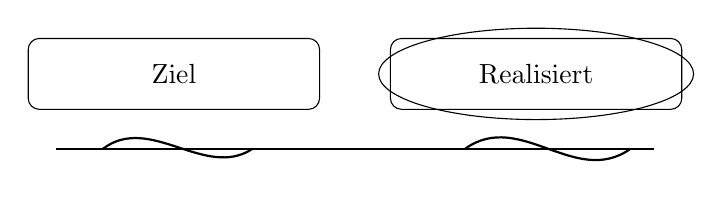
\begin{tikzpicture}[box/.style={draw, rounded corners, minimum width=3.7cm, minimum height=0.9cm, align=center}]
  \node[box] (target) at (-2.3,0) {Ziel};
  \node[box] (real) at (2.3,0) {Realisiert};
  \draw[thick] (-3.8,-0.95) -- (3.8,-0.95);
  \draw[thick] (-3.2,-0.95) .. controls (-2.6,-0.5) and (-1.9,-1.35) .. (-1.3,-0.95);
  \draw[thick] (1.4,-0.95) .. controls (2.1,-0.45) and (2.8,-1.45) .. (3.5,-0.95);
  \draw[thin] (2.3,0) ellipse (2.0cm and 0.58cm);
\end{tikzpicture}

\caption{Unterstützender Vergleich: Ziel- und realisierter Zustand sind verbundene, aber nicht identische Ebenen.}
\label{fig:support-target-vs-realized}
\end{figure}

Daraus folgt, dass jede nachgelagerte Bewertung als ausdrücklicher
Ziel--Realisiert-Vergleich und nicht als stillschweigende Annahme geometrischer
Identität formuliert werden muss.

\section{Komponenten des realisierten Zustands}

\begin{definition}[Realisierte räumliche Trajektorie]
\label{def:realized-spatial-trajectory}
Die realisierte räumliche Trajektorie wird bezeichnet durch
\[
\Gamma_{\mathrm{real}}(s).
\]
\end{definition}

\begin{definition}[Realisierte Krümmung]
\label{def:realized-pose3-curvature}
\[
\kappa_{\mathrm{real}}(s)=\frac{\dd\theta_{\mathrm{real}}}{\dd s}.
\]
\end{definition}

\begin{definition}[Realisierte Überhöhung]
\label{def:realized-cant}
\[
\phi_{\mathrm{real}}(s).
\]
\end{definition}

Im Allgemeinen gilt
\[
\mathrm{pose3}_{\mathrm{real}}
\neq
\mathrm{pose3}_{\mathrm{target}}.
\]

\section{Laufzeitrekonstruktion des realisierten pose3}

Realisiertes pose3 wird typischerweise zur Laufzeit aus beobachteten Daten,
Realisierungsmodellen und Einbettungskontext rekonstruiert.

\begin{definition}[Realisierungsrekonstruktion zur Laufzeit]
\label{def:runtime-realization-reconstruction}
Eine schematische Form lautet
\[
\mathrm{pose3}_{\mathrm{real}}(s)
=
\mathcal E_{\mathrm{real}}(s,x_{\mathrm{target}},m,\mathcal R,\mathcal C),
\]
wobei \(m\) Beobachtungsdaten, \(\mathcal R\) Informationen des
Realisierungsmodells und \(\mathcal C\) den Metrik- und Koordinatenkontext
bezeichnet.
\end{definition}

\begin{principle}[Mehrdeutigkeit des gemessenen Zustands]
\label{princ:measured-state-ambiguity}
Messdaten sind Evidenz für realisiertes pose3, nicht das realisierte pose3
selbst.
\end{principle}

\section{Beobachtungsoperatoren und Sensorintegration}

\begin{definition}[Sensorbeobachtungsmodell]
\label{def:sensor-observation-model}
\[
y_i
=
\mathcal H_i\bigl(\mathrm{pose3}_{\mathrm{real}}(s_i)\bigr)
+
\varepsilon_i,
\]
wobei \(\mathcal H_i\) ein Sensorbeobachtungsoperator und
\(\varepsilon_i\) der Beobachtungsfehler ist.
\end{definition}

Die Inferenz des realisierten Zustands ist somit ein inverses
Rekonstruktionsproblem aus heterogenen Beobachtungen.

Die zweite Abbildung beantwortet die Evidenzfrage: Wie vermittelt beobachtete
Evidenz die Bewertung, statt kanonische Zielbedeutung zu ersetzen?

\begin{figure}[ht]
\centering
% figures/reality/support_target_observed_assessment-DE.tex
\begin{tikzpicture}[
  node distance=1.25cm,
  box/.style={draw, rounded corners, minimum width=4.5cm, minimum height=0.85cm, align=center},
  arrow/.style={->, thick}
]
  \node[box] (t) {Ziel};
  \node[box, below=of t] (o) {Beobachtet};
  \node[box, below=of o] (a) {Bewertung};
  \draw[arrow] (t) -- (o);
  \draw[arrow] (o) -- (a);
  \draw[dashed, thin] ($(o.center)+(0,0)$) ellipse (2.45cm and 0.62cm);
\end{tikzpicture}

\caption{Unterstützende Realisierungssicht: Bewertung hängt von beobachteter Evidenz relativ zur Zielsemantik ab.}
\label{fig:support-target-observed-assessment}
\end{figure}

Die methodische Folge lautet: Beobachtung tritt als Evidenz in eine
Bewertungskette ein. Modellvalidierung muss daher die Trennung zwischen
Zielsemantik, realisiertem Zustand und gemessener Approximation bewahren.

\section{Dynamische Vergleichsgrößen}

\begin{definition}[Realisierte Gleichgewichtsbedingung]
\label{def:realized-equilibrium-condition}
Ein realisiertes Gleis ist dynamisch ausgeglichen, wenn
\[
v^2\kappa_{\mathrm{real}}(s)=g\sin\phi_{\mathrm{real}}(s).
\]
\end{definition}

\begin{definition}[Realisierte effektive Querbeschleunigung]
\label{def:realized-effective-lateral-acceleration}
\[
a_{\mathrm{eff,real}}(s)
=
v^2\kappa_{\mathrm{real}}(s)-g\sin\phi_{\mathrm{real}}(s).
\]
\end{definition}

\begin{definition}[Realisierter Ruck]
\label{def:realized-jerk}
\[
j_{\mathrm{real}}(s)
=
v^3\kappa'_{\mathrm{real}}(s)-gv\cos\phi_{\mathrm{real}}(s)\,\phi'_{\mathrm{real}}(s).
\]
\end{definition}

Diese Größen unterstützen den ingenieurtechnischen Ziel--Realisiert-Vergleich
über reine Positionsabweichung hinaus.

\section{Realisierungsoperator auf pose3}

\begin{definition}[pose3-Realisierungsoperator]
\label{def:pose3-realization-operator}
\[
\mathcal R_{\mathrm{pose3}}:
\mathrm{pose3}_{\mathrm{target}}
\mapsto
\mathrm{pose3}_{\mathrm{real}}.
\]
\end{definition}

Dieser Operator wirkt auf die vollständige Interpretation des
Eisenbahnzustands -- Geometrie, Rahmen, Überhöhung und abgeleitetes dynamisches
Verhalten -- und nicht allein auf Koordinaten.

\section{Verbindung zu AIM}

\begin{summary}
Realisiertes pose3 ist die zentrale Vergleichsebene zwischen
ingenieurtechnischem Zielzustand und beobachteter Eisenbahnrealität.

In AIM wahrt das Kapitel die Trennung zwischen Ziel-, realisiertem und
gemessenem Zustand und verwendet zugleich die kanonischen pose3- und
Realisierungsoperatoren der vorangehenden Teile.
\end{summary}
